% Created 2022-06-14 Tue 19:56
% Intended LaTeX compiler: xelatex
\documentclass[11pt,twoside,landscape]{article}
\usepackage{graphicx}
\usepackage{longtable}
\usepackage{wrapfig}
\usepackage{rotating}
\usepackage[normalem]{ulem}
\usepackage{amsmath}
\usepackage{amssymb}
\usepackage{capt-of}
\usepackage{hyperref}
\usepackage{subcaption}
\usepackage[newfloat]{minted}
\usepackage{color}
\usepackage{listings}
\usepackage[top=2cm,bottom=2cm,right=2cm,left=2cm,landscape]{geometry}
\usepackage{multicol}
\usepackage{enumitem}
\usepackage{fancyhdr}
\usepackage{caption}
\usepackage{algorithm}
\usepackage{algpseudocode}
\setlist{noitemsep}
\setlength{\parindent}{0pt}
\setlength{\columnseprule}{0.2pt}
\definecolor{mygreen}{rgb}{0,0.6,0}
\definecolor{mygray}{rgb}{0.5,0.5,0.5}
\definecolor{mymauve}{rgb}{0.58,0,0.82}
\lstset{ backgroundcolor=\color{white}, basicstyle=\footnotesize, breaklines=true, captionpos=b, commentstyle=\color{mygreen}, escapeinside={\%*}{*)},keywordstyle=\color{blue}, stringstyle=\color{mymauve},}
\usepackage{caption}
\author{Olivier Lischer}
\date{\today}
\title{MsTe Summary}
\hypersetup{
 pdfauthor={Olivier Lischer},
 pdftitle={MsTe Summary},
 pdfkeywords={},
 pdfsubject={},
 pdfcreator={Emacs 28.1 (Org mode 9.5.4)}, 
 pdflang={English}}
\begin{document}

\pagestyle{fancy}
\fancyhf{}
\fancyhead[R]{MsTe-HS21}
\fancyhead[L]{Exam Summary}
\fancyfoot[CE,CO]{\leftmark}
\fancyfoot[R]{\thepage}
\fancyfoot[L]{Olivier Lischer}
\begin{multicols}{3}

\section{Wohlstand}
\label{sec:org33ef26a}
\subparagraph{Der einfache Wirtschafskreislauf} \
\label{sec:org0d29813}

{
\begin{center}
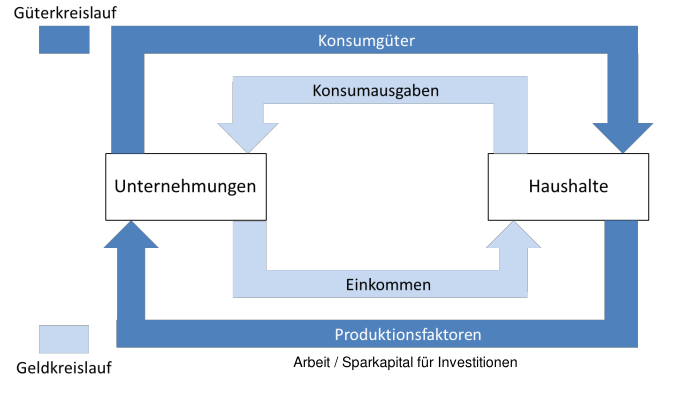
\includegraphics[width=.9\linewidth]{img/wirtschaftskreislauf.png}
\end{center}
\captionof{figure}{Der einfache Wirtschaftskreislauf}\label{fig:einfache-wirtschaftskreislauf}
}

\subparagraph{Der erweiterte Wirschaftskreislauf} \
\label{sec:org49446dd}
{
\begin{center}
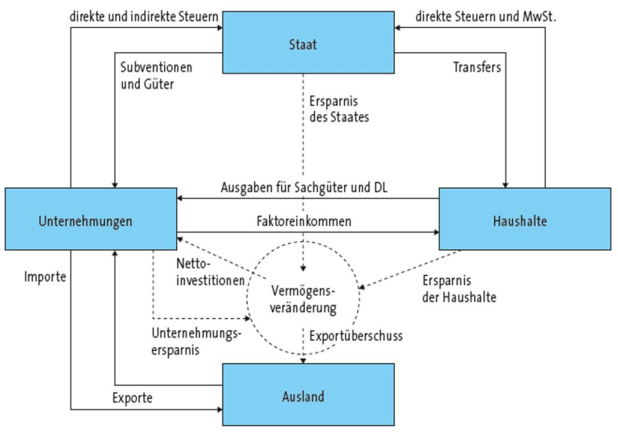
\includegraphics[width=.9\linewidth]{img/wirtschaftskreislauf_erweitert.png}
\end{center}
\captionof{figure}{Der erweiterte Wirschaftskreislauf}\label{fig:erweiterte-wirschaftskreislauf}
}

\subparagraph{Was ist Wohlstand} \
\label{sec:orgb169e2e}
Wohlstand ist dasselbe wie das BIP (Bruttoinlandprodukt, \href{../../../roam/20220504151208-was_ist_das_bip.org}{Was ist das BIP?}).

\subparagraph{Was ist das BIP?} \
\label{sec:org63008ad}
BIP ist nicht anders als Wohlstand (\href{../../../roam/20220504150706-was_ist_wohlstand.org}{Was ist Wohlstand?}).
Interessant: Beamtenlöhne entsprechen dem Produktionswert des Staats und fliesen daher ins BIP ein.


Das BIP gibt es als:
\begin{itemize}
\item Nominales BIP (Standard BIP = Produktionswert - Vorleistung)
\item Reales BIP (Referenzjahr)
\item BIP pro Kopf
\item Kaufkraftbereinigtes BIP (BIP auf einen internationalen Standard beglichen)
\end{itemize}

{
\begin{center}
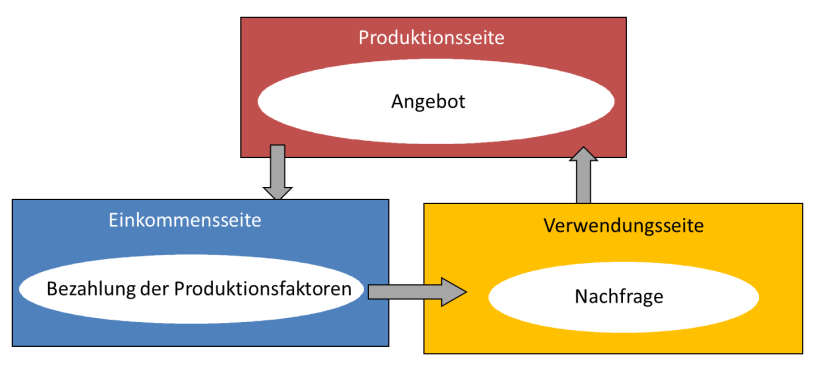
\includegraphics[width=.9\linewidth]{img/bip_blickwinkel.png}
\end{center}
\captionof{figure}{Die drei Blickwinkel des BIPs}\label{fig:drei-blickwinkel-bips}
}


\subparagraph{Die volkswirtschaftlichen Produktionsfaktoren} \
\label{sec:orga1d6b8c}
\begin{itemize}
\item Arbeit - Menschen
\item Kapital - Maschine, Gebäuden, Infrastruktur
\item Technologien
\item Boden / natürliche Ressourcen
\end{itemize}

\section{End}
\label{sec:org3e5cafe}
\end{multicols}
\end{document}